\chapter{Communication}
A communication system is desired for transporting the GoT data, calculated to coordinates on the computer, to the microcontroller, located on the vehicle. Furthermore a protocol handling packet transitions is necessary to implement on top of the communication system to be able to fulfil requirements set in \secref{sec:Requirements}.

% The har two Xbee radio modules. The communication setup for the Xbee modules will be explained in this chapter.

\section{OSI model}
The Open Systems Interconnection, OSI, model is a standard used to describe how information moves in a network. Each layer describing standardization of what should occur in the specific layer. The seven layers of the OSI model can be seen in \tableref{tab:OSIModel}.

\begin{table}[H]\centering
\begin{tabular}{|p{1.5cm}|p{3cm}|}
\hline%-----------------------------------------------------------------------------------------------------------------
  \textbf{Layer} & \textbf{OSI} \\
\hline%-----------------------------------------------------------------------------------------------------------------
    7 &    Application      \\
\hline%-----------------------------------------------------------------------------------------------------------------
    6 &    Presentation      \\
\hline%-----------------------------------------------------------------------------------------------------------------
    5 &    Session       \\
\hline%-----------------------------------------------------------------------------------------------------------------
    4 &    Transport    \\
\hline%-----------------------------------------------------------------------------------------------------------------
    3 &   Network     \\
\hline%-----------------------------------------------------------------------------------------------------------------
    2 &   Data link     \\
\hline%-----------------------------------------------------------------------------------------------------------------
    1 &    Physical     \\
\hline%-----------------------------------------------------------------------------------------------------------------
\end{tabular}
\caption{OSI model}
\label{tab:OSIModel}
\end{table}

An overall description of the main functionalities in the different layers is examined and a description of what layers are utilized for in the prototypes communication protocol, is given:

The Physical layer is the electrical/mechanical hardware layer. The layer handles bits and determines what is a binary 0 and 1. The prototype utilizes two Xbee's, one in the computer and one on the vehicle, for the lowest layer of communication.

The Data link layer functionality ensures physical addressing, error control when transferring data between node over the physical layer and access control \cite{JensMyerSlides}. The Data link layer is something the Xbee module handles to ensure a byte is send correctly \todo{Check up on that}.

The Network layers main functionality is routing across a network. This is not utilized in the protocol. Since to communication is only between two modules. 

The Transport layers handles packets and can assemble or disassemble packets if necessary. An important part of the functionality of this layer is to ensure reliable transmission of data packets.

  

 




%Notes:
%We use UDP, no connections

%OSI
%The physical layer is the Xbee
%The data link layer is halfway done in the code, where the package is split up in bytes. The adressing is done on the XBee and in the serial port libeary 
%The network layer may not be used here as we just transmit 360 degree
%The transport layer is the setup of how the package is setup
%The rest of the layers is not used.


\section{Transport Layer}

%is made to understand what contains each byte sent from the transmitter to the receiver. The use of a protocol for the transport layer will make sure that each end of the communication system understand how each package of bytes is build up.

The main object for the communication system is to send the coordinates from the computer to the microcontroller. A transport layer protocol is created to ensure packets can be transmitted, receive, i.e. extract the needed information from the packet, and to identify erroneous packets.

A connectionless system is implemented, since it is one-way communication, from the computer to the microcontroller and retransmission not desired, since the vehicle is moving and a retransmission of a coordinate will cause a delay. Additionally, the sampling rate of the GoT system i 10 \si{Hz}, so transmitting the recently received coordinates would be sufficient. Therefore is erroneous packages thrown away and acknowledgements is not utilized.

\subsection{Protocol Package Structure}
A package structure is desired for containing necessary information for addressing, decrypting and error handling. The protocol has an header which contains a start byte, a destination and the length of the package. The body of the package is the data and the tail is the checksum and the end byte. The order of the package structure is illustrated in \tableref{CoorSetup}.

\begin{table}[H]\centering
\begin{tabular}{|>{\centering\arraybackslash}m{2cm}|>{\centering\arraybackslash}m{3cm}|>{\centering\arraybackslash}m{2cm}|>{\centering\arraybackslash}m{2cm}|>{\centering\arraybackslash}m{2cm}|>{\centering\arraybackslash}m{2cm}|}
\multicolumn{6}{c}{12 Byte} \\
\hline
Start Byte & Destination ID & length & Data & Checksum & End byte \\
\hline
\end{tabular}
\caption{The structure of a package}
\label{CoorSetup}
\end{table}

\textbf{Destination ID} is to ensure packages, which is transmitted, is handled by the correct receiver. This way the transmitter can transmit to numerous receivers if multiple vehicles is utilized. The destination ID ensures the receivers can filter out packages not intended for them. The microcontroller has the destination ID 0000 0001. The length of the destination byte is set to one byte, so the destination can be read immediately when received.

UDP, a connectionless protocol, utilizes a source, but in this case it is not necessary, since only one computer is transmitting, the receiver does not need to know where the package has been transmitted from. Even if there more computers was utilized it would not be necessary as long as the package is marked with the destination ID, the receivers is able to read it. If retransmission was utilized, in case of erroneous packages, a source is necessary to have the ability to ask for a retransmission from the sender. Since retransmission is not utilized a source is not included in the package structure.

\textbf{Length} is utilized by the receiver. This will make it possible for the receiver to know the bit length of the package, and thereby know when the package should end. Each package created has the same length. The length is set to contain 7 bit, this can count up to $2^{7}-1 = 127$, which is sufficient.

\subsubsection{Data}
The data received from the GoT system consist of three coordinates (X,Y,Z), locating the position of the vehicle. Each of these coordinates can have a value from -9000 to 9000 (See \appref{GoTDescription}). To contain a number of this size, a 15 bit signed integer is utilized. Of the 15 bit 14 bit is utilized for the magnitude of the coordinate, which can have a value of 16385 ($2^{14}-1$). The last bit of the 15 bit is utilized to indicate if a coordinate is positive or negative, i.e. sign bit. The protocol is designed so the sign bit will be placed at the end of the 15 bit integer. As both the microcontroller and the computer utilizes little endians, there will not be a problem with the transmission of numbers. With little endians, the bit with the highest value will be located next to the sign bit and the bit with the lowest value is located at the beginning of the bit array. This will yield the bit array illustrated on \tableref{CoorSetup}.

\begin{table}[H]
\centering
\begin{tabular}{|>{\centering\arraybackslash}m{0.5cm}|>{\centering\arraybackslash}m{0.5cm}|>{\centering\arraybackslash}m{0.5cm}|>{\centering\arraybackslash}m{0.5cm}|>{\centering\arraybackslash}m{0.5cm}|>{\centering\arraybackslash}m{0.5cm}|>{\centering\arraybackslash}m{0.5cm}|>{\centering\arraybackslash}m{0.5cm}|>{\centering\arraybackslash}m{0.5cm}|>{\centering\arraybackslash}m{0.5cm}|>{\centering\arraybackslash}m{0.5cm}|>{\centering\arraybackslash}m{0.5cm}|>{\centering\arraybackslash}m{0.5cm}|>{\centering\arraybackslash}m{0.5cm}|>{\centering\arraybackslash}m{0.65cm}|}
\multicolumn{15}{c}{15 bits} \\
\hline
$2^0$ & $2^1$ & $2^2$ & $2^3$ & $2^4$ & $2^5$ & $2^6$ & $2^7$ & $2^8$ & $2^9$ & $2^{10}$ & $2^{11}$ & $2^{12}$ & $2^{13}$ & $+/-$ \\
\hline
\end{tabular}
\caption{Setup for the bit array, that contains one of the coordinate values.}
\label{CoorSetup}
\end{table}

The representation of the integer is called signed magnitude. Another representation that could be used is ones' complement. Here the number is inverted if the signed bit is true. But for an easier implementation on the computer, the signed magnitude is utilized. The code firsts checks if the number is positive or negative. If negative, the sign bit is set and the number is multiplied by minus one, this will yield the magnitude. The magnitude is then converted into a bit array. When converting back, it is only necessary to multiply the magnitude by minus one, if the sign bit is true.

\subsubsection{Checksum}
To ensure package data is received correctly, error handling is added to the protocol. A error handling which is utilized is a checksum. The way the checksum is calculated, is by splitting the header and the data up into pieces of equal size and then summing the pieces together. The summed bit array is then inverted and the remaining bit array is the checksum. 

there is 60 bit in the header and the data combined, i.e. 15 per coordinate, 8 for the destination and 7 for the length. these will be split up into three pieces of 20 bit. The related checksum consist of 20 bit. Combined, the header, data and checksum is 80 bit, which is equal to 10 bytes. In \tableref{ChecksumExp} an example of calculating a checksum is given.

\begin{table}[H]
\centering
\begin{tabular}{c c c c c c c c c c c}
   & Bit array  &     & Decimal &     & Bit 0-3 & Bit 4-7 & Bit 8-11 & Bit 12-15 & Bit 16-19 & Bit 20 \\
\hline
a) & Part 1     & $=$ & 123008  & $=$ & 0000 & 0001 & 0000 & 0111 & 1000 & \\
b) & Part 2     & $=$ & 351365  & $=$ & 1010 & 0001 & 0011 & 1010 & 1010 & \\
c) & Part 3     & $=$ & 729671  & $=$ & 1110 & 0010 & 0100 & 0100 & 1101 & \\
d) & Part 1+2+3 & $=$ & 1204044 & $=$ & 0011 & 0010 & 1111 & 1010 & 0100 & 1 \\
e) & Add carry  & $=$ & 155469  & $=$ & 1011 & 0010 & 1111 & 1010 & 0100 & \\
f) & Checksum   & $=$ & 893106  & $=$ & 0100 & 1101 & 0000 & 0101 & 1011 & \\
g) & Check      & $=$ & 1048575 & $=$ & 1111 & 1111 & 1111 & 1111 & 1111 & \\
\end{tabular}
\caption{The pieces consisting of the destination ??, length with the value of 96, and the data which is 4259, 7511 and -6418.}
\label{ChecksumExp}
\end{table}

The three pieces is added together, the destination, length and the data (see on line d). This produces a carry, since the checksum has the size of 20 bit. The carry is added to the beginning of the sum (see on line e). The generated sum is then inverted to yield a checksum (sees on line f).

When the receiver utilizes the checksum needs to check if the destination, length and data corresponds with the related checksum. The checksum is first added together with the three 20 bit pieces and, if there is any, the carry. If the outcome of the bit summation results in 20 bits which are true, then the package is received correctly. If not, the receiver will throw away the package. An error in the received package could be a bit inversion or some data not received by the receiver. 

A flaw when utilizing the created checksum, is that an error can cancelled out another error, and thereby make the errors undetectable. This can happen when the system adds the three pieces and the checksum together. An example, is if the first bit in piece number one is true and the first bit in piece number two is false. If both of these bits are shifted independently, so the bit from part one become false and the bit in part two true, the checksum can not detect the error. The likelihood for this to happen is very slim, as the errors first have to occur and then they have to be located a place where they cancel each other out. Having only 4 pieces of 20 bits, the likelihood of this happening is lesser than if the checksum was set to 10 bit. Since the addition occurs with 7 pieces of 10 bit. This would yield more bits with the same rank, so there would be a higher possibility for a bit cancelling each other out. This is a good argument for utilizing a larger checksum, even if it uses more space.

\subsubsection{Start and end byte}

As the GOT system send a package each time it makes a measurement of the coordinates, a queue of package can appear in the Arduino, if it does not read fast enough. This can confuse the system which may not differenciate the package from each other. It can be avoided by adding a start byte at the start of the package and an end byte at the end. 

When the system wants to find the start of the package, it will search for the start byte. When finding this byte, it will read the header, data and checksum and then look for the end byte. If the end byte is not there, it means that the package was not received correctly and is thrown away. If the end byte is there, the system will take the whole package and apply the error handling on it. 

The start byte will be set to 0000 1111. This is chosen so that the start byte can not have the same value as one of the other bytes in the header, so these will not be misunderstood as the start byte. To have the start and end byte as different as possible, as the end byte will come just before the next start byte, the end byte is the inverted number of the start byte, which is 1111 0000.


With the data, header, checksum, start and end byte, a package will look like the illustration on \tableref{PackageLook}

\begin{table}[H]
\centering
\begin{tabular}{|c|c|>{\centering\arraybackslash}m{0.3cm}|>{\centering\arraybackslash}m{0.3cm}|>{\centering\arraybackslash}m{0.3cm}|>{\centering\arraybackslash}m{0.3cm}|>{\centering\arraybackslash}m{0.3cm}|>{\centering\arraybackslash}m{0.3cm}|>{\centering\arraybackslash}m{0.3cm}|>{\centering\arraybackslash}m{0.3cm}|>{\centering\arraybackslash}m{0.3cm}|>{\centering\arraybackslash}m{0.3cm}|>{\centering\arraybackslash}m{0.3cm}|>{\centering\arraybackslash}m{0.3cm}|>{\centering\arraybackslash}m{0.3cm}|>{\centering\arraybackslash}m{0.3cm}|>{\centering\arraybackslash}m{0.3cm}|>{\centering\arraybackslash}m{0.3cm}|}
\hline
\multicolumn{2}{|c|}{Offsets} & \multicolumn{8}{c}{Byte 1} & \multicolumn{8}{|c|}{Byte 2} \\
\hline
\multicolumn{1}{|c}{Byte} & \multicolumn{1}{|c|}{Bit} & 0 & 1 & 2 & 3 & 4 & 5 & 6 & 7 & 8 & 9 & 10 & 11 & 12 & 13 & 14 & 15 \\
\hline
0 & 0 & \multicolumn{8}{c}{Start byte} & \multicolumn{8}{|c|}{Destination} \\
\hline
2 & 16 & \multicolumn{7}{c}{Length} & \multicolumn{9}{|c|}{X coordinate} \\
\hline
4 & 32 & \multicolumn{6}{c}{X coordinate} & \multicolumn{10}{|c|}{Y coordinate} \\
\hline
6 & 48 & \multicolumn{5}{c}{Y coordinate} & \multicolumn{11}{|c|}{Z coordinate} \\
\hline
8 & 64 & \multicolumn{4}{c}{Z coordinate} & \multicolumn{12}{|c|}{Checksum} \\
\hline
10 & 80 & \multicolumn{8}{c}{Checksum} & \multicolumn{8}{|c|}{End byte} \\
\hline
\end{tabular}
\caption{Illustration of a package, that will be send from the transmitter to the receiver.}
\label{PackageLook}
\end{table}

This gives a package length of 96 bit (12 byte). As the GoT system have a sampling frequency of 10 Hertz and each sampling gives out 12 byte, the transfer speed for the Xbee have to be greater than 120 byte per second. 

\subsubsection{Error handling}
As there is a chance that the package is getting damaged under the way from the transmitter to the receiver, some error handling is used to check the packages for error and throw the damage packages away. One of these is the checksum, which is explained further up in this section. Besides the checksum, the start and end byte is used to see if the number of byte received is right, according to the length in the header.

But as with the checksum, where there is a flaw if there are multiples errors and these cancel each other out in the control, there is a flaw in the error handling for receiving packages. The receiving process can be seen on \figref{FlowReceiver}.

%\begin{figure}[H]
%\centering
%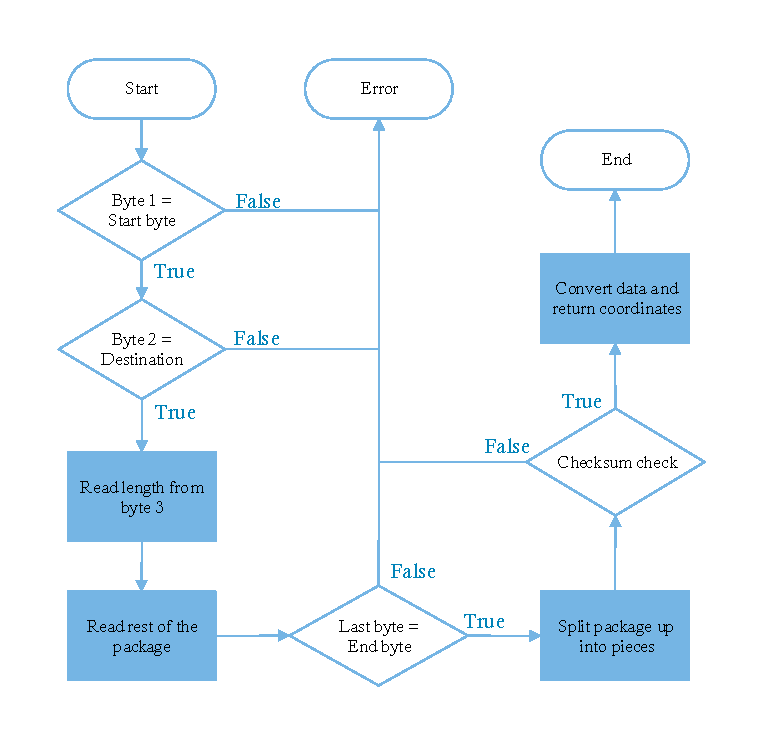
\includegraphics[scale=0.7]{figures/FlowReceiver.pdf}
%\caption{Flow chart over the error handling in the receiver part.}
%\label{FlowReceiver}
%\end{figure}

If the package is transmitted correctly, the 1st byte will be the start byte, the 2nd byte will be the destination ID of the receiver. The 3rd byte will contain 7 bit for the length and 1 bit for the first coordinate. If the length is correct, it will be 96, which is 12 byte. The last byte, the 12th one, is the end byte. Then if these condition are all correct, the receiver will make a control with the checksum. If that one is also correct, the system will convert the data and return the coordinates to the rest of the system.

If there is an error, then all the bytes that have been read will be thrown away. This is because the bytes are taken from the buffer of the receiving Xbee and can not be put back at the same place, after being taken out. So if the start byte and the destination are correct, but the end byte is not, the whole package is thrown away. If the start byte is not correct, then only that byte will be thrown away until finding a correct one. This method is applied because the system can only work with complete packages.

This prevents the receiver to start in the middle of a package, as the system will just throw away the bad package, until it finds the start byte. A problem that comes with this feature, is that as the start byte is only on a normal byte, a byte in the data or the checksum part can have the same value. If the receiver then by fault beginning looks after the start byte in these part and find a byte equal to the start byte, it can consider the 9 next bytes as a package. The problem will first happen if the byte afterwards is equal to the receiver's destination ID, and the first seven bits of the next byte are equal to 96. An example on a situation where this problem happens can be seen on \tableref{errorPro}.

\begin{table}[H]
\centering
\begin{tabular}{c | m{0.1cm} m{0.1cm} m{0.1cm} m{0.1cm} m{0.1cm} m{0.1cm} m{0.1cm} m{0.1cm} | c | m{0.1cm} m{0.1cm} m{0.1cm} m{0.1cm} m{0.1cm} m{0.1cm} m{0.1cm} m{0.1cm} | l }
\multicolumn{9}{c}{Normal reading} & \multicolumn{9}{c}{Displaced reading} &  \\
\cline{2-9} \cline{11-18}
1st byte & 0 & 0 & 0 & 0 & 1 & 1 & 1 & 1 & 5th byte & 0 & 0 & 0 & 0 & 1 & 1 & 1 & 1 & $\leftarrow$ Start byte \\
\cline{2-9} \cline{11-18}
2nd byte & 0 & 0 & 0 & 0 & 0 & 0 & 0 & 1 & 6th byte & 0 & 0 & 0 & 0 & 0 & 0 & 0 & 1 & $\leftarrow$ Destination \\
\cline{2-9} \cline{11-18}
3rd byte & 0 & 0 & 0 & 0 & 0 & 1 & 1 & 0 & 7th byte & 0 & 0 & 0 & 0 & 0 & 1 & 1 & 0 & $\leftarrow$ Length (First seven bit)\\
\cline{2-9} \cline{11-18}
4th byte & 1 & 1 & 1 & 1 & 0 & 0 & 0 & 0 & 8th byte & 0 & 1 & 1 & 1 & 0 & 0 & 1 & 1 & \\
\cline{2-9} \cline{11-18}
5th byte & 0 & 0 & 0 & 0 & 1 & 1 & 1 & 1 & 9th byte & 1 & 0 & 0 & 1 & 1 & 0 & 1 & 1 & \\
\cline{2-9} \cline{11-18}
6th byte & 0 & 0 & 0 & 0 & 0 & 0 & 0 & 1 & 10th byte & 1 & 0 & 0 & 0 & 0 & 1 & 0 & 0 & \\
\cline{2-9} \cline{11-18}
7th byte & 0 & 0 & 0 & 0 & 0 & 1 & 1 & 0 & 11th byte & 0 & 0 & 1 & 1 & 0 & 1 & 1 & 1 & \\
\cline{2-9} \cline{11-18}
8th byte & 0 & 1 & 1 & 1 & 0 & 0 & 1 & 1 & 12th byte & 1 & 1 & 1 & 1 & 0 & 0 & 0 & 0 & \\
\cline{2-9} \cline{11-18}
9th byte & 1 & 0 & 0 & 1 & 1 & 0 & 1 & 1 & 1st byte & 0 & 0 & 0 & 0 & 1 & 1 & 1 & 1 & \\
\cline{2-9} \cline{11-18}
10th byte & 1 & 0 & 0 & 0 & 0 & 1 & 0 & 0 & 2nd byte & 0 & 0 & 0 & 0 & 0 & 0 & 0 & 1 & \\
\cline{2-9} \cline{11-18}
11th byte & 0 & 0 & 1 & 1 & 0 & 1 & 1 & 1 & 3rd byte & 0 & 0 & 0 & 0 & 0 & 1 & 1 & 0 & \\
\cline{2-9} \cline{11-18}
12th byte & 1 & 1 & 1 & 1 & 0 & 0 & 0 & 0 & 4th byte & 1 & 1 & 1 & 1 & 0 & 0 & 0 & 0 & $\leftarrow$ End byte\\
\cline{2-9} \cline{11-18}
\end{tabular}
\caption{Example of a normal reading of a package and a displaced reading of a package. The package contains the coordinates (-8222, 515, -3699). For the displaced reading, another package equal to the first one comes after the first package.}
\label{errorPro}
\end{table}

For the example on \tableref{errorPro}, the 5th to 7th byte are equal to the start byte and the header. So if the system is looking after the start byte and find the 5th byte, before it finds the next 1st byte, it will begin to look for the header. In this case it will find it and as the 12th byte, which is in the next package, is equal to the end byte, the system will consider it have founded a complete package. But as there is also the control with the checksum, the package will probably not go through the security system. The checksum, in this case, will not be the original checksum for the package, but another part of the package. As this checksum is not calculated to fit, the chance for the check goes through is so small that it will not be considerer to happen. 

But even if the wrong package is being stopped by the control with the checksum, the 12 bytes still have been read and therefore have to be thrown. This will happen no matter if the end byte is correct or not, just as long as the system finds the start byte and the header. And in these 12 bytes, the next real start byte is also thrown away. In worst case scenario, the next three byte, after the ones that got thrown away, is equal to the start byte and header again, the same scenario will repeat it self and will go on, until the three byte no longer equals the start byte and header.

These scenarios about beginning to read a package in the middle of a package is not that common, as three byte are needed to be precisely like the start byte and the header (the last bit of the third byte is from the x coordinate, so it is not needed to be the same). The chance is small that the data and checksum parts are 8 bytes long together,  and that the system recognize the wrong start byte and header. Even if both things happens, as the coordinate will change for each package because of the moving vehicle, it will not be considered to be happening in a row. And as the system do not have a problem with one package missing, this flaw in the error handling will not considered as a problem.



The protocol of the Xbee modules are now explained and implemented, with the handling errors

